% !TEX program = xelatex
\documentclass[10pt,letterpaper,twocolumn]{article}
\usepackage[margin=.65in]{geometry}
\usepackage{fontspec}
\setmainfont{Latin Modern Roman}[Extension=.otf,UprightFont=lmroman10-regular,BoldFont=lmroman10-bold,ItalicFont=lmroman10-italic,BoldItalicFont=lmroman10-bolditalic]
\setsansfont{Latin Modern Sans}[Extension=.otf,UprightFont=lmsans10-regular,BoldFont=lmsans10-bold,ItalicFont=lmsans10-oblique]
\setmonofont{Latin Modern Mono}[Extension=.otf,UprightFont=lmmono10-regular,ItalicFont=lmmono10-italic,Scale=.85]
\newfontfamily\acbold{ywft-processing-bold}[Path=../../system/public/type/webfonts/,Extension=.ttf]
\usepackage{xcolor,booktabs,tabularx,enumitem,graphicx,tikz,balance,hyperref,xurl,microtype}
\usetikzlibrary{arrows.meta,positioning}
\usepackage{ac-source-bundle}
\definecolor{acpink}{RGB}{180,72,135}
\definecolor{acink}{RGB}{29,37,57}
\definecolor{acblue}{RGB}{37,100,128}
\newcommand{\ac}{Aesthetic{\color{acpink}.}Computer}
\hypersetup{colorlinks=true,urlcolor=acblue,linkcolor=acblue,citecolor=acblue,pdfauthor={@jeffrey},pdftitle={The Score and the Session}}
\setlength{\columnsep}{.25in}
\setlength{\emergencystretch}{1.5em}
\setlist[itemize]{leftmargin=*,nosep}
\setlist[enumerate]{leftmargin=*,itemsep=2pt}
\newcommand{\file}[1]{\texttt{\path{#1}}}
\begin{document}
\twocolumn[\begin{center}
{\acbold\LARGE The Score and the Session\par}
\vspace{5pt}
{\large Instructions, shared terms, and daily work in \ac}\par
\vspace{6pt}
@jeffrey\quad\small ORCID: 0009-0007-4460-4913\par
September 15, 2026\par
\end{center}
\begin{abstract}
Repository instructions serve a continuing working relationship as well as individual coding tasks. We combine a repository audit, empirical studies, recent release incidents, and a bounded review of authorized prompt history and tool traces in \ac. The initial diagnosis---uneven instruction discovery and duplicated operational authority---holds, but a shorter score is insufficient. Daily work depends on shared terms, visual inspection, parallel sessions, and resuming unfinished tasks across hosts. Published experiments also give mixed results for instruction files, using different success and efficiency endpoints. We propose a small stable policy, explicit workflow definitions, selective context preloading, and refreshed session state, with executable evidence at completion. These are testable design recommendations; the audit does not measure their productivity effect.
\end{abstract}\vspace{10pt}]

\section{Problem and precedent}
A recent Oskiewar release appeared complete, then disappeared when production returned to an older version from another branch. This incident motivates an audit of how instructions connect user intent, repository state, and verified completion.

The user introduced \emph{compushloy}: always commit, push, and deploy. Its amended definition also requires the intended deployment branch and verification of the pushed revision. That amendment is the only shared-policy change made during this analysis. The broader restructuring below remains a proposal.

The earlier \emph{Reading the Score} criticized a document serving too many audiences and proposed a conductor's score with separate parts~\cite{reading}. We retain that distinction, but change the test: can the current tools actually find the right part, and can a reader establish that its requested action completed? The current public Platter and relevant local sources were consulted before drafting~\cite{platter}.

\section{Method and observed inventory}
We inspected tracked paths, symlinks, instructions, and deployment code. A separate subagent performed a read-only audit. The primary agent checked findings and official loader documentation. Root instruction files match between working HEAD \file{275329e763ab} and fetched production main \file{a97038281a06}; the terminology amendment is additionally present locally.

\begin{table}[ht]
\centering\small
\begin{tabularx}{\columnwidth}{@{}lrrX@{}}
\toprule
Entry & Lines & Bytes & Observed role\\
\midrule
SCORE.md & 738 & 42,689 & Shared policy and reference\\
AGENTS.md & --- & --- & Symlink to SCORE.md\\
CLAUDE.md & 161 & 9,882 & Separate Claude guide\\
CODEX.md & --- & --- & Absent\\
\bottomrule
\end{tabularx}
\caption{Working-copy inventory on September 15. The symlink is an entry path, not another independent text. Exact hashes and nested paths accompany the paper in inventory.json.}
\label{tab:inventory}
\end{table}

There are 22 tracked files with exact basename \file{SCORE.md}, including the root, one nested \file{CLAUDE.md}, and no nested \file{AGENTS.md}. The repository has no tracked \file{CODEX.md} or local \file{.codex/} directory in the inspected tree.

Evidence locations, consultation notes, and exclusions are recorded in \file{notes.md}.

\begin{figure*}[t]
\centering
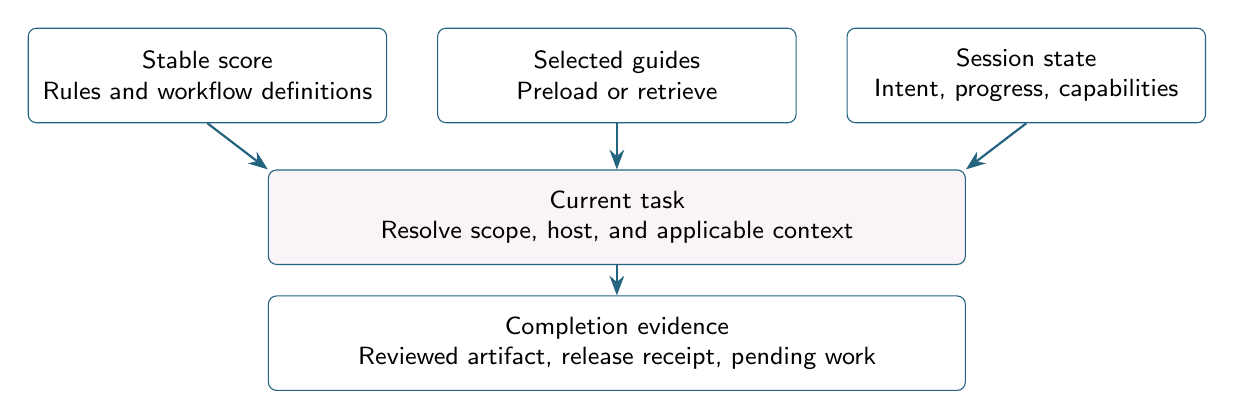
\begin{tikzpicture}[font=\sffamily\small,box/.style={draw=acblue,rounded corners=3pt,align=center,minimum height=12mm,text width=42mm,inner sep=5pt},flow/.style={-{Stealth[length=2.5mm]},thick,draw=acblue}]
\node[box] (policy) at (-5.2,0) {Stable score\\Rules and workflow definitions};
\node[box] (guides) at (0,0) {Selected guides\\Preload or retrieve};
\node[box] (state) at (5.2,0) {Session state\\Intent, progress, capabilities};
\node[box,text width=85mm,fill=acpink!6] (task) at (0,-1.8) {Current task\\Resolve scope, host, and applicable context};
\node[box,text width=85mm] (evidence) at (0,-3.4) {Completion evidence\\Reviewed artifact, release receipt, pending work};
\draw[flow] (policy.south) -- (task.north west);
\draw[flow] (guides.south) -- (task.north);
\draw[flow] (state.south) -- (task.north east);
\draw[flow] (task.south) -- (evidence.north);
\end{tikzpicture}
\caption{Proposed working context. Stable policy, selected references, and refreshed state meet at the task. A later handoff carries progress and evidence while rechecking host-dependent assumptions. These routes supplement each tool's instruction loader.}
\label{fig:routes}
\end{figure*}

\section{What the empirical evidence supports}
Gloaguen et al.'s revised study evaluates 300 SWE-bench Lite tasks and 138 CTXbench tasks across four agent/model configurations~\cite{gloaguen}. Neither generated nor developer-provided files significantly improve test-based success over no file in its aggregate comparisons. Developer files outperform generated files ($p=0.038$); generated files increase average inference cost by 20\% and 23\% on the two benchmarks. Length and instruction-category ablations also fail to establish a strong performance effect. This directly weakens a blanket ``shorter is better'' claim. The study uses one completion per configuration and Python-focused tasks, including generated specifications and tests. It does not measure our release, design, or handoff outcomes.

Lulla et al. report a different result in paired runs on 124 PR tasks from 10 repositories using gpt-5.2-codex~\cite{lulla}: median time to final output falls from 98.57 to 70.34 seconds with AGENTS.md, a 28.64\% relative reduction. Median output tokens fall 16.58\%. The sample requires one root instruction file and small code-only changes. Fifty tasks receive a qualitative output sanity check; systematic semantic correctness is outside scope. Faster final output is therefore evidence about efficiency in that setting, not proof of equivalent completed work. This design excludes the overlapping nested guidance central to our case.

METR's early-2025 randomized trial covers 16 experienced developers and 246 tasks in familiar repositories; AI access increased completion time by 19\% despite perceived speedups~\cite{metr}. Its February 2026 follow-up warns that selection effects and concurrent-agent time accounting make newer estimates unreliable~\cite{metrupdate}. Neither study tests our instruction architecture. They motivate measuring human attention, review, and rework alongside agent latency, especially when several prox sessions run concurrently.

A descriptive study of 2,303 context files across 1,925 repositories finds frequent small additions and configuration-like evolution~\cite{readmes}. That is evidence of maintenance pressure, not a causal result about length. Collectively, the literature supports an evaluation question rather than a universal rule: which context prevents a costly mistake on this task, and what extra work does it induce?

\section{Discovery is not a filename metaphor}
Codex documents a root-to-working-directory search, choosing at most one project file per directory: \file{AGENTS.override.md}, then \file{AGENTS.md}, then configured fallback names. Its default combined project budget is 32 KiB~\cite{codex}. Our root score alone exceeds that value by 9,921 bytes. A simulated 32,768-byte prefix ends inside chat-query material at line 504. This demonstrates a default-budget risk; it does not prove this session was truncated. The user supplied score instructions directly, and launch-time overrides were not exhaustively audited.

Claude Code documents \file{CLAUDE.md} loading and explicit \file{@path} imports; its documented shared-AGENTS route uses an import or symlink~\cite{claude}. Our Claude entry instead tells readers in ordinary prose to read the score and ant rules. That can guide an agent's subsequent action, but is not the same mechanism as an explicit import. A fourth filename has no established benefit until a loader consumes it.

Nested scores are similarly an authoring convention rather than a universal discovery mechanism. The papers route is explicit in the root, but there is no complete path-to-score map for all domains.



\section{Where authority has drifted}
Three forms of drift recur. First, scope disagrees: the root calls the ant rules ant-specific, their document says all agents, and Claude directs contributors to both. Unattended colony approval rules can conflict with an already-authorized repair. The active request establishes authorization; colony behavior needs an explicit operating scope.

Second, shared guidance has tool-specific entry points. HAND and SCREEN are routed through Claude, although code style and piece layout apply across agents. The root also misidentifies the root Claude guide as the full piece API reference. Native release recipes differ between local upload and oven workflows; session-server descriptions disagree about hosting. These requirements need one owned source and neutral task routes.

Third, environment guidance arrives late. ENVIRONMENT already resolves explicit identity and observed capabilities before customary editor preferences~\cite{environment}, but the root introduces it after extensive host material. Its heading-scoped Emacs block also leaves subsequent helper lists formally untagged. Move the resolver early and bound editor-specific procedures explicitly.

\section{Completion needs executable evidence}
\subsection{The deployment incident}
The observed sequence was: feature-branch v120 served correctly; a later public read returned v118 even with a cache-busting URL; the server checkout was \file{main}; the fixes were integrated with newer main changes; v122 was pushed to main and deployed. Identity, gzip, and Brotli responses then matched the intended source. We did not identify the actor initiating the intervening deployment. The evidence supports a publication-branch mismatch, not a browser-cache explanation or a causal claim about one paragraph of instructions.

The deployment script's default target is its current checkout branch, with an explicit override available~\cite{release}. A transient successful deploy therefore does not prove that the next routine deploy will retain the change. The release contract must name both the artifact and the branch that owns production.

\subsection{Tracked hooks versus installed hooks}
The audited checkout contains tracked pre-commit policy, but no installed pre-commit hook or configured hooks path; post-commit is linked. A repository file describes a potential enforcement mechanism, not proof that it ran. Source inspection also found an arena push-failure branch that logs a skipped deployment without exiting before the following deployment commands. This is a code-level finding, not a reproduced failed push. A future fix should be verified with a failing transport stub and zero downstream deploy calls.


\section{Daily work changes the unit of analysis}
\subsection{History is a sample, not a complete diary}
At the user's request, we consulted the prompt-history index and native transcript records for recurring terms and tooling. The quantitative window is September 1--14, 2026, UTC, excluding this analysis. Searches recovered two hosts; other configured histories were unavailable. Native call requests and filtered prompt mentions are separate evidence types; neither proves successful execution.

The local extraction uses top-level Claude and Codex transcripts, timestamp filtering, exact repository cwd, and call-ID deduplication. Worktrees, nested cwd, other repositories, and subagent directories are outside that sample. Codex's execution wrapper requires a second accounting layer: a syntactic tool call inside JavaScript is a candidate dispatch, not a confirmed invocation. Sampling details and aggregate results accompany this revision; private transcript text does not.


The native sample contains 8,641 tool-call requests across 83 sessions and 1,216 accepted short prompts. Of those prompts, 439 arrive as structured queued-command attachments; counting ordinary user messages alone misses them. Selected lexical matches include compush in 28 prompts across 19 sessions, prox in 19 across 13, Chrome in 16 across 13, and Easel in 10 across 6. These counts are descriptive and conservative: longer prompts and nested cwd are excluded. They are not a ranking of workflow value.

\begin{table}[ht]
\centering\small
\begin{tabularx}{\columnwidth}{@{}Xrr@{}}
\toprule
Tool family & Native requests & Wrapper sites\\
\midrule
Chrome browser MCP & 867 & 0\\
Puppet MCP & 374 & 19\\
Frame MCP & 21 & 156\\
Paper MCP & 4 & 88\\
Prox MCP & 16 & 13\\
\bottomrule
\end{tabularx}
\caption{Selected local tool families. Wrapper sites are syntactic candidates inside JavaScript, not additional confirmed executions; do not sum the columns. Shell requests are more numerous: 4,541 Bash and 1,617 execution-wrapper requests.}
\end{table}

The separate remote index slice contains compush in 36 short events across 25 sessions and prox in 29 across 21. Coverage and filters differ; those figures are not pooled with native logs. Direct read-only access recovered a host missed by the connector.

\subsection{Shared words carry operational meaning}
The reviewed history repeatedly uses release shorthand, named prox references, requests to inspect a browser, and requests to resume earlier work. A September 13 definition makes oskieploy a release across the game's surfaces. In the current conversation, compushloy explicitly names commit, push, and deploy. These are compact workflow selections, whereas a machine or prox name identifies where the work belongs.

\begin{table}[ht]
\centering\small
\begin{tabularx}{\columnwidth}{@{}lX@{}}
\toprule
Term family & Required interpretation\\
\midrule
compush / compushloy & Distinct release meanings; consult the current explicit definition\\
oskieploy & Game release across named surfaces, with channel status\\
prox / prompt rock & Session reference; resolve identity and unfinished work\\
frame / Chrome & Select the intended visual surface, then inspect it\\
/papers / Platter & Scholarly workflow and evidence, including rendered QA\\
Wordcrust / Slidecop & Editorial and presentation acceptance criteria\\
\bottomrule
\end{tabularx}
\caption{A proposed vocabulary route, not a frequency ranking. Rare terms may still encode essential requirements.}
\end{table}

Keep a small workflow glossary with scope, definition source, implementation entry point, and completion evidence. Similar spellings are useful retrieval candidates, but must not silently expand an action: an old compush request must not acquire a new deployment obligation solely through fuzzy matching. Likewise, frame can mean a screenshot workflow or a game's simulation frame. Resolve the surrounding task before choosing tooling.

The existing Jeffrey Lexicon supplies a useful provenance precedent: first-hand language is separated from generated text~\cite{lexicon}. Operational definitions need an additional distinction: an explicit definition, a repeated usage, and an agent's inferred synonym have different authority. A frequent word is not automatically a rule; a one-time explicit correction can govern the next action. Keep discovered candidates separate from accepted definitions.

\subsection{Inspection and continuity are part of completion}
The history includes a concrete visual loop: inspect a named prox window, adjust the interface, reopen it, and inspect a fresh frame. It also contains requests to recover work after reboot and continue a former prox. These observations make a file-only view of productivity incomplete. A code change may still need a live browser, rendered PDF, physical device, or release receipt before the user's objective is satisfied.

The recent Oskiewar sequence illustrates the same pattern: performance work led into lobby input, theme contrast, start-event consumption, physics, deployment, then process analysis. The domain expanded without a new repository or a clean task boundary. Routes must therefore consider the active request and touched paths, and be reconsidered when the task changes. Cwd inheritance alone cannot cover this workflow.

\section{Proposed instruction architecture}
Keep one short canonical score for stable shared policy, with explicit routes to owned guides. Separate four kinds of information: rules that apply across tasks, definitions of named workflows, task-specific reference material, and live session state. They have different owners and update rates. A source-tree overview can be rediscovered; the meaning of compushloy or a previously accepted correction may not be recoverable from code.


\file{AGENTS.md} can remain the symlink where it works. Claude can import the same short score and retain only genuinely tool-specific additions. Cross-platform environments unable to preserve symlinks need an explicitly generated adapter with a drift check. A \file{CODEX.md} may be a linked human reference, but should not be introduced as a second authority or assumed startup file.

Nested scores need explicit path triggers. Merely splitting a large root into named files will not make those files load. Routes should cover piece authoring, runtime work, service release, native devices, papers, and host tools. Match both task intent and touched paths. Loader behavior and follow-up reads are separate mechanisms; naming another file does not ensure either.


\subsection{Preload repeated work; retrieve uncommon detail}
Easel deliberately inlines selected authoring guides from the checkout or its packaged context~\cite{bundle}. This is a local counterexample to deferring all detail. For repeated piece work, preload a bounded authoring bundle with source revision and freshness checks. For an occasional service repair, retrieve that service's guide. The 8 KiB root target is a proposed guardrail, not an empirical optimum; neither byte count nor link count measures usefulness.

\subsection{Reconcile state when work resumes}
A prox handoff should retain the objective, accepted corrections, relevant definitions, worktree/revision, completed evidence, pending channels, and next action. On the receiving host, refresh actual cwd, capabilities, and resource constraints. Preserve user intent while rechecking machine-dependent assumptions. The current prox bundle records identity, cwd, and provider but lacks explicit revision and instruction digests; its resume script can fall back to the home directory~\cite{prox}. This is a schema observation, not proof that a particular handoff failed.

Easel also documents a state gap: an autopublish toggle changes UI behavior immediately but reaches the model on a new thread. Such changes need a short state update during the task, rather than another permanent paragraph in SCORE. State reconciliation should trigger on a real transition, not add a ritual before every edit.

\subsection{Enforce shared release state outside prose}
Recent commits repair worktree receipt placement and compressed-artifact rebuilding in the webhook path~\cite{releasefixes}. They show why one reviewed command cannot represent all production writers. Inventory the CLI, webhook, and hooks; align their branch and artifact contracts. Atomic receipt replacement prevents partial JSON, but concurrent releases may still overwrite one another's desired revision. That race is a hypothesis requiring a fixture. A release lease or revision-checked update belongs in execution tooling, while the score states the requirement.

\section{Migration and evaluation plan}
\begin{enumerate}
\item Freeze an inventory and mark each requirement's owner, scope, and consumers. Keep exact safety and authorization semantics before editing prose.
\item Extract long operational sections into owned guides. Keep essential entry guidance within a proposed 8 KiB budget, leaving room for nested instructions. This is a design target, not a measured optimum.
\item Reduce tool adapters and validate links, symlinks, import targets, and duplicated controlled definitions. Easel's explicit context-bundle inventory and check mode provide a local implementation precedent~\cite{bundle}.
\item Define release records: target service, canonical branch, command, expected source revision, served-artifact check, and pending channels. Distinguish pushed, published, device-accepted, and physically verified states.
\item Test fresh sessions from the root and representative subdirectories. Verify which instructions loaded and which guides were subsequently read; do not infer this from filenames alone.
\end{enumerate}

An instruction doctor should be read-only by default. It should report missing or stale adapters, budget overruns, broken route links, installed-hook state, and conflicting controlled terms. It should neither install hooks nor upload session text as a side effect of checking instructions.

Start with paired replays of held-out tasks: piece authoring, browser-visible repair, a prox handoff, papers QA, and a multi-surface release. Compare the current entry with a concise entry plus a selected preload; then vary eager versus lazy loading separately. Keep mandatory constraints identical. Pin repository snapshots, model/harness versions, capabilities, and cache conditions; repeat runs rather than attributing one stochastic result to the file.

Judge completion against task-specific evidence, not an agent's final answer. Record correction turns, repeated discovery, review/rework, agent elapsed time, and sampled human active time separately. Concurrent sessions make summed wall-clock time misleading. A historical replay may already be familiar to the model, so reserve prospective tasks for confirmation. Use transport stubs and artifact fixtures for release experiments; do not benchmark by repeatedly deploying production. No such intervention trial has been run here.

\section{Limits, privacy, and conclusion}
This dated audit does not establish fleet-wide discovery, hook installation elsewhere, model attention, or an optimal instruction budget. User context can bypass normal discovery. Static contradictions do not establish runtime failures; fresh-agent trials remain future work.

Authorized prompt history and native call records were consulted for this revision. Correspondence and credentials were outside scope. The paper retains operational aggregates and paraphrased workflow observations; raw transcripts, identifiers, and command arguments remain excluded from its source bundle. Native and indexed samples are not pooled. Prompt authorship filters and wrapper extraction are imperfect, and the history cannot identify causal productivity effects. Drafting and audit assistance were provided by Codex, with a separate subagent review.

The recommended update is a stable shared score supported by a workflow glossary, selected task context, refreshed session state, and executable completion evidence. Shortening the entry can remove duplication; preserving the working relationship is the larger design problem.

\balance
\begin{thebibliography}{99}\small
\bibitem{score} @jeffrey. Root score and instruction adapters. Repository snapshots and working amendment, September 2026. Evidence inventory and paths in \file{notes.md}.
\bibitem{reading} @jeffrey. \emph{Reading the Score: A Critical Analysis of SCORE.md as Governance, Interface, and Creative Form}. 2026. \file{papers/arxiv-score-analysis/score-analysis.tex}.
\bibitem{codex} OpenAI. \emph{Custom instructions with AGENTS.md}. Accessed September 15, 2026. \url{https://learn.chatgpt.com/docs/agent-configuration/agents-md}.
\bibitem{claude} Anthropic. \emph{How Claude remembers your project}. Accessed September 15, 2026. \url{https://code.claude.com/docs/en/memory}.
\bibitem{environment} @jeffrey. \emph{Execution Environments}. \file{ENVIRONMENT.md}, lines 13--41. Inspected September 2026.
\bibitem{release} @jeffrey. Deployment and release implementations. \file{lith/deploy.fish}, \file{.githooks/post-commit}, and \file{xbox/tools/oskiewar-release.mjs}. Snapshots identified in consultation notes.
\bibitem{platter} @jeffrey. \emph{Research Platter}. Rendered index and local papers score, consulted September 15, 2026. \url{https://papers.aesthetic.computer/platter.html}.
\bibitem{bundle} @jeffrey. Easel context synchronization. \file{easel/bin/sync-context.mjs}, explicit inventory and check mode. 2026.
\bibitem{gloaguen} T. Gloaguen et al. \emph{Evaluating AGENTS.md: Are Repository-Level Context Files Helpful for Coding Agents?} 2026. \url{https://arxiv.org/abs/2602.11988v2}.
\bibitem{lulla} J. L. Lulla et al. \emph{On the Impact of AGENTS.md Files on the Efficiency of AI Coding Agents}. 2026. \url{https://arxiv.org/abs/2601.20404v2}.
\bibitem{metr} J. Becker et al. \emph{Measuring the Impact of Early-2025 AI on Experienced Open-Source Developer Productivity}. 2025. \url{https://arxiv.org/abs/2507.09089v1}.
\bibitem{metrupdate} J. Becker et al. \emph{We are Changing our Developer Productivity Experiment Design}. February 24, 2026. \url{https://metr.org/blog/2026-02-24-uplift-update/}.
\bibitem{readmes} W. Chatlatanagulchai et al. \emph{Agent READMEs: An Empirical Study of Context Files for Agentic Coding}. 2025. \url{https://arxiv.org/abs/2511.12884v1}.
\bibitem{lexicon} @jeffrey. Jeffrey Lexicon. \file{papers/jeffrey-lexicon/README.md} and \file{manifest.json}. Consulted September 15, 2026.
\bibitem{prox} @jeffrey. Prox bundle and resume implementation. \file{slab/bin/prox-mcp.mjs}, bundle metadata and resume-script generation. Audited snapshot in notes.
\bibitem{releasefixes} @jeffrey. Release worktree and webhook corrections. Commits \file{3b1496c428} and \file{135d05d311}; Easel context/state handling in fetched main. See notes.
\end{thebibliography}
\end{document}
